\chapter{Data}
\label{chap:data}

% review once background is done (reference equations, usw)
\section{\textit{Herschel} column-density maps}
\subsection{Introduction}
The main source of data in this work stems from ESA's \textit{Herschel} Space Observatory \cite{pilbratt2010herschel}, which was launched in 2009 with the goal of observing in the far-infrared and submillimetre wavelengths. 
\textit{Herschel} was equipped with three main instruments: the Photodetector Array Camera and Spectrometer (PACS), the Spectral and Photometric Imaging Receiver (SPIRE), and the Heterodyne Instrument for the Far Infrared (HIFI). These instruments allowed \textit{Herschel} to observe a wide range of astronomical phenomena, including star formation and galaxy evolution.
\textit{Herschel}'s mission lasted until 2013, enabling unprecedented studies of the cold and dusty regions of space.

%introduction to Orion's data
\textit{Herschel}'s observations of Orion, the target of this work, were part of the \textit{Herschel} Gould Belt Survey (HGBS). This survey aimed to map the nearby star-forming regions in the Gould Belt, a flat structure of a few hundred parsecs inclined by approximately 20$^{\circ}$ with respect to the galactic plane \cite{andre2010herschel}.
The clouds covered by the HGBS span a wide range of physical and environmental conditions, from very active, cluster-forming complexes such as the Orion A and B giant molecular clouds (GMCs) to quiescent regions with no star formation activity at all.

\subsection{Dust emission maps}
In the interstellar medium, dust typically has temperatures T$_{\mathrm{dust}}$ around $20$ K and emits thermal radiation that can be approximated by a modified blackbody, peaking at far-infrared (FIR) and submillimetre (mm) wavelengths. 
This thermal dust emission represents the dominant source of FIR and mm-continuum radiation in galaxies, as it can be recognized in Figure \ref{fig:dust_emission_blackbody}. 

\begin{figure}
    \centering
    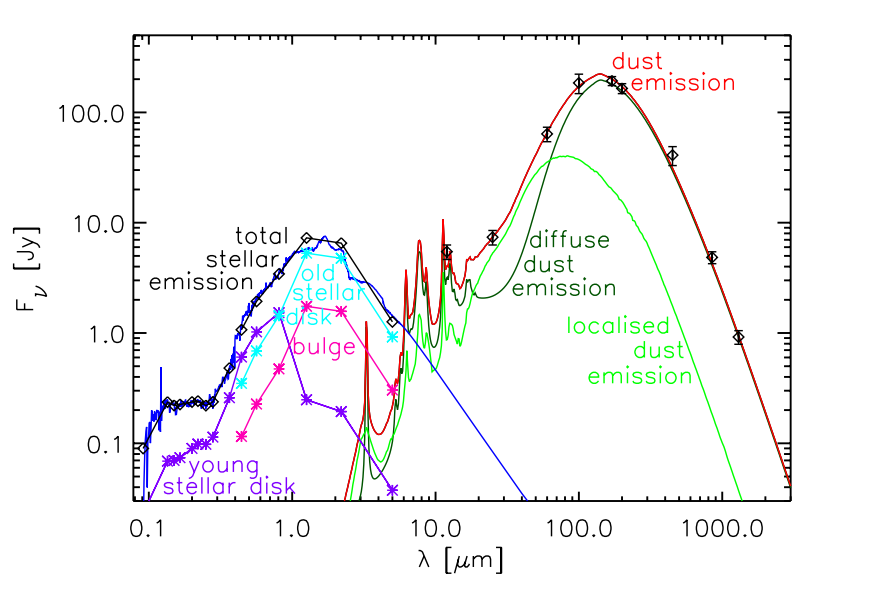
\includegraphics[width=0.75\textwidth]{figures/dust_emission_blackbody.png}
    \caption{Best fit SED of NGC 891 and observed data in infrared and submillimeter. Also plotted are the main components responsible for each part of the emission spectrum \cite{popescu2011modelling}. Dust emission represents the dominant source of FIR and mm-continuum radiation in galaxies.}
    \label{fig:dust_emission_blackbody}
\end{figure}

Dust grains absorb ultraviolet (UV) and near-infrared (NIR) photons from stars, reprocessing this stellar radiation and re-emitting it at longer wavelengths. 
Because dust is highly efficient at radiating energy, it reaches and maintains relatively low equilibrium temperatures \cite{hildebrand1983determination}. 
Observations of dust emission hence provide a powerful tool to estimate the column density of dust and gas along the line of sight.

Using mm continuum dust emission to measure column density offers several advantages over traditional extinction-based methods: it can probe much higher column densities where extinction becomes saturated or unreliable, it often provides better angular resolution, and it remains effective even in regions heavily obscured by dust where extinction mapping fails \cite{draine2003interstellar}. Moreover, continuum observations allow simultaneous determination of both dust temperature (T$_{\mathrm{dust}}$) and gas column density (N(H$_2$)), which is essential for characterizing dense molecular clouds. In extragalactic studies, where individual stars cannot be resolved, dust emission often represents the only viable method for estimating gas masses.

However, these methods also involve significant assumptions and uncertainties. Different approaches to estimate column density are conceptually equivalent but may yield different results due to methodological degeneracies. One key source of uncertainty arises from the poorly constrained dust opacity, $\kappa$, which depends on the composition, size distribution, and physical properties of dust grains. Variations in $\kappa$ directly affect the derived column densities, introducing systematic uncertainties into the analysis.

The data used in this work are \textit{Herschel} column-density maps of the Orion A and B giant molecular clouds. These maps were created by combining data from PACS and SPIRE instruments, which observed at different wavelengths to capture the dust emission across the clouds.

Specifically, PACS provided imaging photometry in the 60-210 $\mu m$ wavelength range, using two filled silicon bolometer arrays with 16 $\times$ 32 and 32 $\times$ 64 pixels. In photometric mode, PACS simultaneously imaged two bands: either 60-85 $\mu m$ or 85-125 $\mu m$, along with 125-210 $\mu m$, covering a field of view of approximately 1.75 $\times$ 3.5 arcminutes with near-Nyquist sampling \cite{poglitsch2010photodetector}. These bands are particularly sensitive to warmer dust components.

SPIRE extended the coverage to longer wavelengths, better tracing colder dust. Its photometer operated in three broad bands centered at 250 $\mu m$, 350 $\mu m$, and 500 $\mu m$, well-suited for mapping large-scale dust emission from the cold interstellar medium \cite{griffin2010herschel}. 

The combination of PACS and SPIRE photometric data allows for the characterization of the dust spectral energy distribution (SED) across a broad range of temperatures. The relative throughputs of the two instruments can be seen in Figure \ref{fig:pacs_spire_throughputs}, on top of black body radiation for typical temperatures of dust. This broad wavelength coverage enables accurate fitting of modified blackbody models to derive dust temperatures, column densities, and emissivity properties.

% Mabye more on the above once you describe better the process below
\begin{figure}
    \centering
    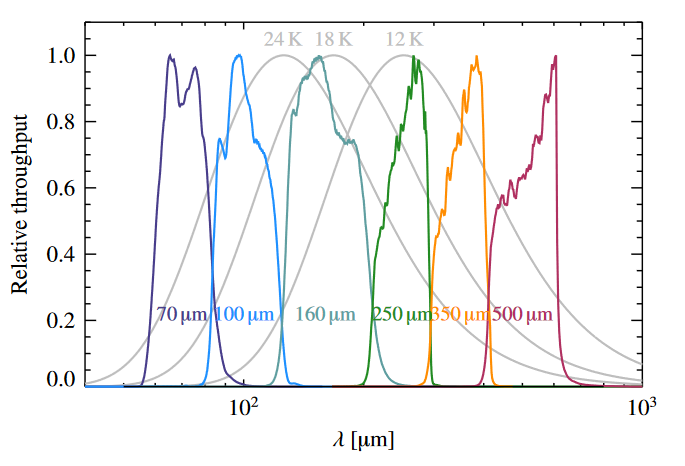
\includegraphics[width=0.75\textwidth]{figures/relative_throughputs_PACS_SPIRE.png}
    \caption{Throughputs in relative units of the PACS and SPIRE bands and three modified blackbodies for typical dust temperatures (12 K, 18 K, 24 K) and with $\beta$ = 1.8 \cite{lombardi2014herschel}.}
    \label{fig:pacs_spire_throughputs}
\end{figure}

% To-Do:
% Give range of N and compare it to the given one in Lombardi 2014 (DONE)
% Maybe also the range in mag
% Mention low res planck data

\subsection{Derivation of column density maps}

To derive the column density maps of the Orion A and B molecular clouds, we used the extinction maps produced by \cite{lombardi2014herschel}, which are publicly available through the CDS Archive\footnote{\href{https://cdsarc.cds.unistra.fr/viz-bin/cat/J/A+A/566/A45\#/browse}{Orion optical-depth and column-density maps: J/A+A/566/A45 (CDS)}}. 
These maps were constructed by fitting the dust emission data from Herschel PACS and SPIRE instruments to a modified blackbody model, providing estimates of the optical depth at 353 GHz ($\tau_{353}$), along with the associated uncertainty maps.

The data products consist of multi-plane FITS files where PLANE1 corresponds to the optical depth map at 353 GHz, and PLANE2 contains the pixel-wise uncertainties. Each map header includes metadata describing projection parameters, coordinate coverage, and the empirical calibration parameters used in the conversion from dust optical depth to extinction, and subsequently to column density. The effective resolution of these maps is 36 arcsec, with pixel dimensions of $3444 \times 2492$, covering both Orion A and B clouds. The given resolution excludes the Planck data, which is at a lower resolution of 5 arcmin.

Following the approach in \cite{lombardi2014herschel}, we converted the optical depth maps into $K$-band extinction maps ($A_K$) using a linear relation of the form:

\begin{equation}
    A_K = \gamma \cdot \tau_{353} + \delta
    \label{eq:ak_tau_relation}
\end{equation}

The constants $\gamma$ and $\delta$ were calibrated separately for Orion A and B using near-infrared extinction data from the 2MASS/NICEST method \cite{lombardi2009nicest}. Specifically:
\begin{itemize}
    \item For Orion A, $\gamma = 2640$ mag and $\delta = 0.012$ mag.
    \item For Orion B, $\gamma = 3460$ mag and $\delta = -0.001$ mag.
\end{itemize}

\begin{figure}[t]
    \centering
    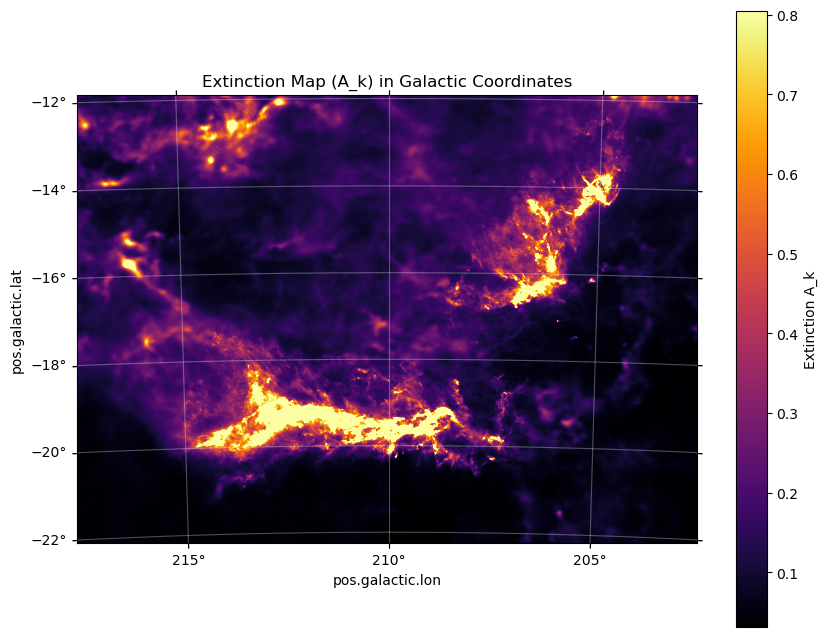
\includegraphics[width=0.75\textwidth]{figures/extinction_map.png}
    \caption{Extinction map of Orion A and B derived from Herschel data, showing the extinction in K-band ($A_V$) across the clouds. The map is based on the optical depth at 353 GHz, converted to extinction using the relation in Equation \ref{eq:ak_tau_relation}.}
    \label{fig:extinction_map}
\end{figure}

The $A_K$ extinction map can be seen in Figure \ref{fig:extinction_map}. 
To convert from $A_K$ to visual extinction $A_V$, we assumed a standard extinction curve with $R_V = 3.1$, following \cite{bohlin1978survey} and \cite{rieke1985interstellar}, giving:

\begin{equation}
    A_V = \frac{A_K}{0.112}
    \label{eq:av_ak_relation}
\end{equation}

Finally, assuming all hydrogen is in molecular form (i.e., fully in H$_2$) and a standard gas-to-dust ratio, the column density of molecular hydrogen was derived using:

\begin{equation}
    N(\mathrm{H_2}) = 0.93 \times 10^{21} \cdot A_V [cm^{-2}]
    \label{eq:n_h2_av_relation}
\end{equation}

\begin{figure}[t]
    \centering
    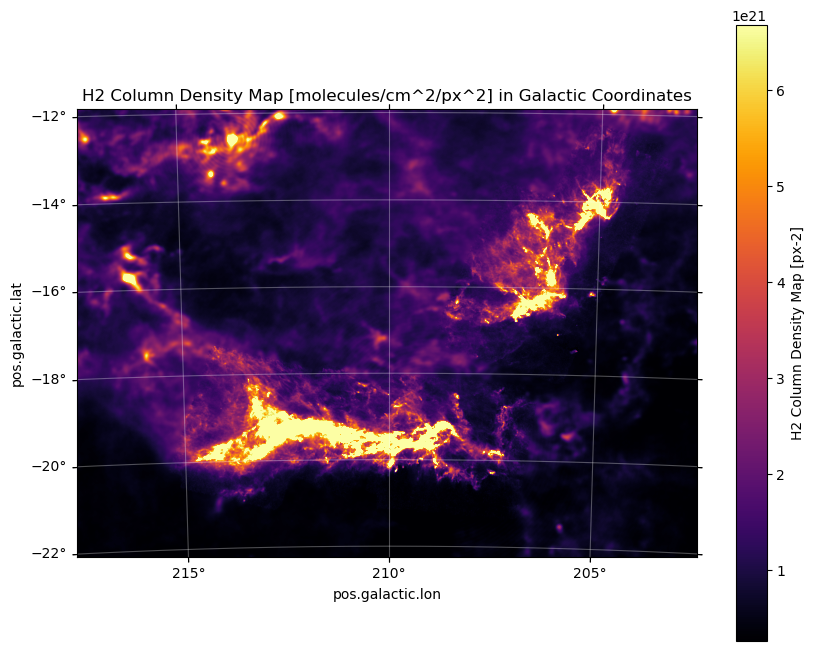
\includegraphics[width=0.75\textwidth]{figures/column_density_map.png}
    \caption{Column density maps of the Orion Complex derived from Herschel data, showing the total column density of molecular hydrogen $N(\mathrm{H}_2)$ across the cloud. The maps are based on the optical depth at 353 GHz.}
    \label{fig:n_h2_final_map}
\end{figure}

The derived column density maps of the Orion Complex can be seen in Figure \ref{fig:n_h2_final_map}. The $H_2$ column density ranges from around 10$^{21}$ cm$^{-2}$ to a few $10^{23}$ cm$^{-2}$ (REVIEW), conferming the specification in the literature \cite{lombardi2014herschel}. 

This method provides a robust, emission-based estimate of the total column density across Orion A and B, with the advantage of tracing both high and low column density regions uniformly.
However, it is important to note that the derivation relies on assumptions about dust properties, uniform opacity, and gas-to-dust ratio, which introduce systematic uncertainties into the absolute calibration of $N(\mathrm{H}_2)$.

% To-Do:
% Add 8.56e33
% Add definition of Orion A and B clouds (DONE)
% Change colour blue of Orion B
% Add "Orion A" and "Orion B" labels
% Colour bar as big as the map (or rather vice versa)
% Add some properties of the mass map (range, sum, mean, std, etc.)

\subsubsection{Derivation of Mass Maps}

Mass maps are a crucial component in this work, allowing us to estimate the total mass of the Orion A and B molecular clouds and their substructures. These maps are computed directly from the H$_2$ column density maps derived in the previous section, by converting the number of molecules per unit area into a mass per pixel.

The conversion process follows these steps:

\begin{enumerate}
    \item \textbf{Pixel area conversion:} \\
    Each pixel in the column density map subtends a solid angle on the sky, which is converted into a physical area based on the known distance to the Orion complex, assumed to be $D = 412$ pc. The pixel scale is 0.00417$^\circ$/px, which is first converted to radians and then used to compute the physical pixel size:

    \[
    \theta_{\mathrm{px}} = \frac{\mathrm{pixel\_scale}}{180/\pi}, \quad 
    \mathrm{px\_size\ (pc)} = \sin(\theta_{\mathrm{px}}) \cdot D
    \]

    The area per pixel in cm$^2$ is then obtained by converting parsecs to centimeters:

    \[
    \mathrm{Area_{px}} = \mathrm{px\_size}^2 \times (3.086 \times 10^{18}\,\mathrm{cm/pc})^2
    \]

    \item \textbf{Column density to mass:} \\
    The H$_2$ column density $N(\mathrm{H}_2)$ in cm$^{-2}$ is multiplied by the pixel area to yield the number of molecules per pixel. This is then converted to mass using the proton mass, $m_p = 1.673 \times 10^{-27}$ kg, and the mean molecular weight correction factor ($\mu = 2.8$) to include helium and heavier elements.:

    \[
    M_{\mathrm{H}_2} = N(\mathrm{H}_2) \cdot \mathrm{Area_{px}} \cdot 2.8 \cdot m_p
    \]

    \item \textbf{Conversion to solar masses:} \\
    The result is then converted from kilograms to solar masses using:

    \[
    M_{\mathrm{px}} = \frac{M_{\mathrm{H}_2}}{M_\odot}, \quad \text{with } M_\odot = 1.9885 \times 10^{30}\, \mathrm{kg}
    \]
\end{enumerate}

The resulting mass map provides the total H$_2$ mass contained in each pixel of the map, with units of solar masses and can be seen in Figure \ref{fig:mass_map}.

\begin{figure}[t]
    \centering
    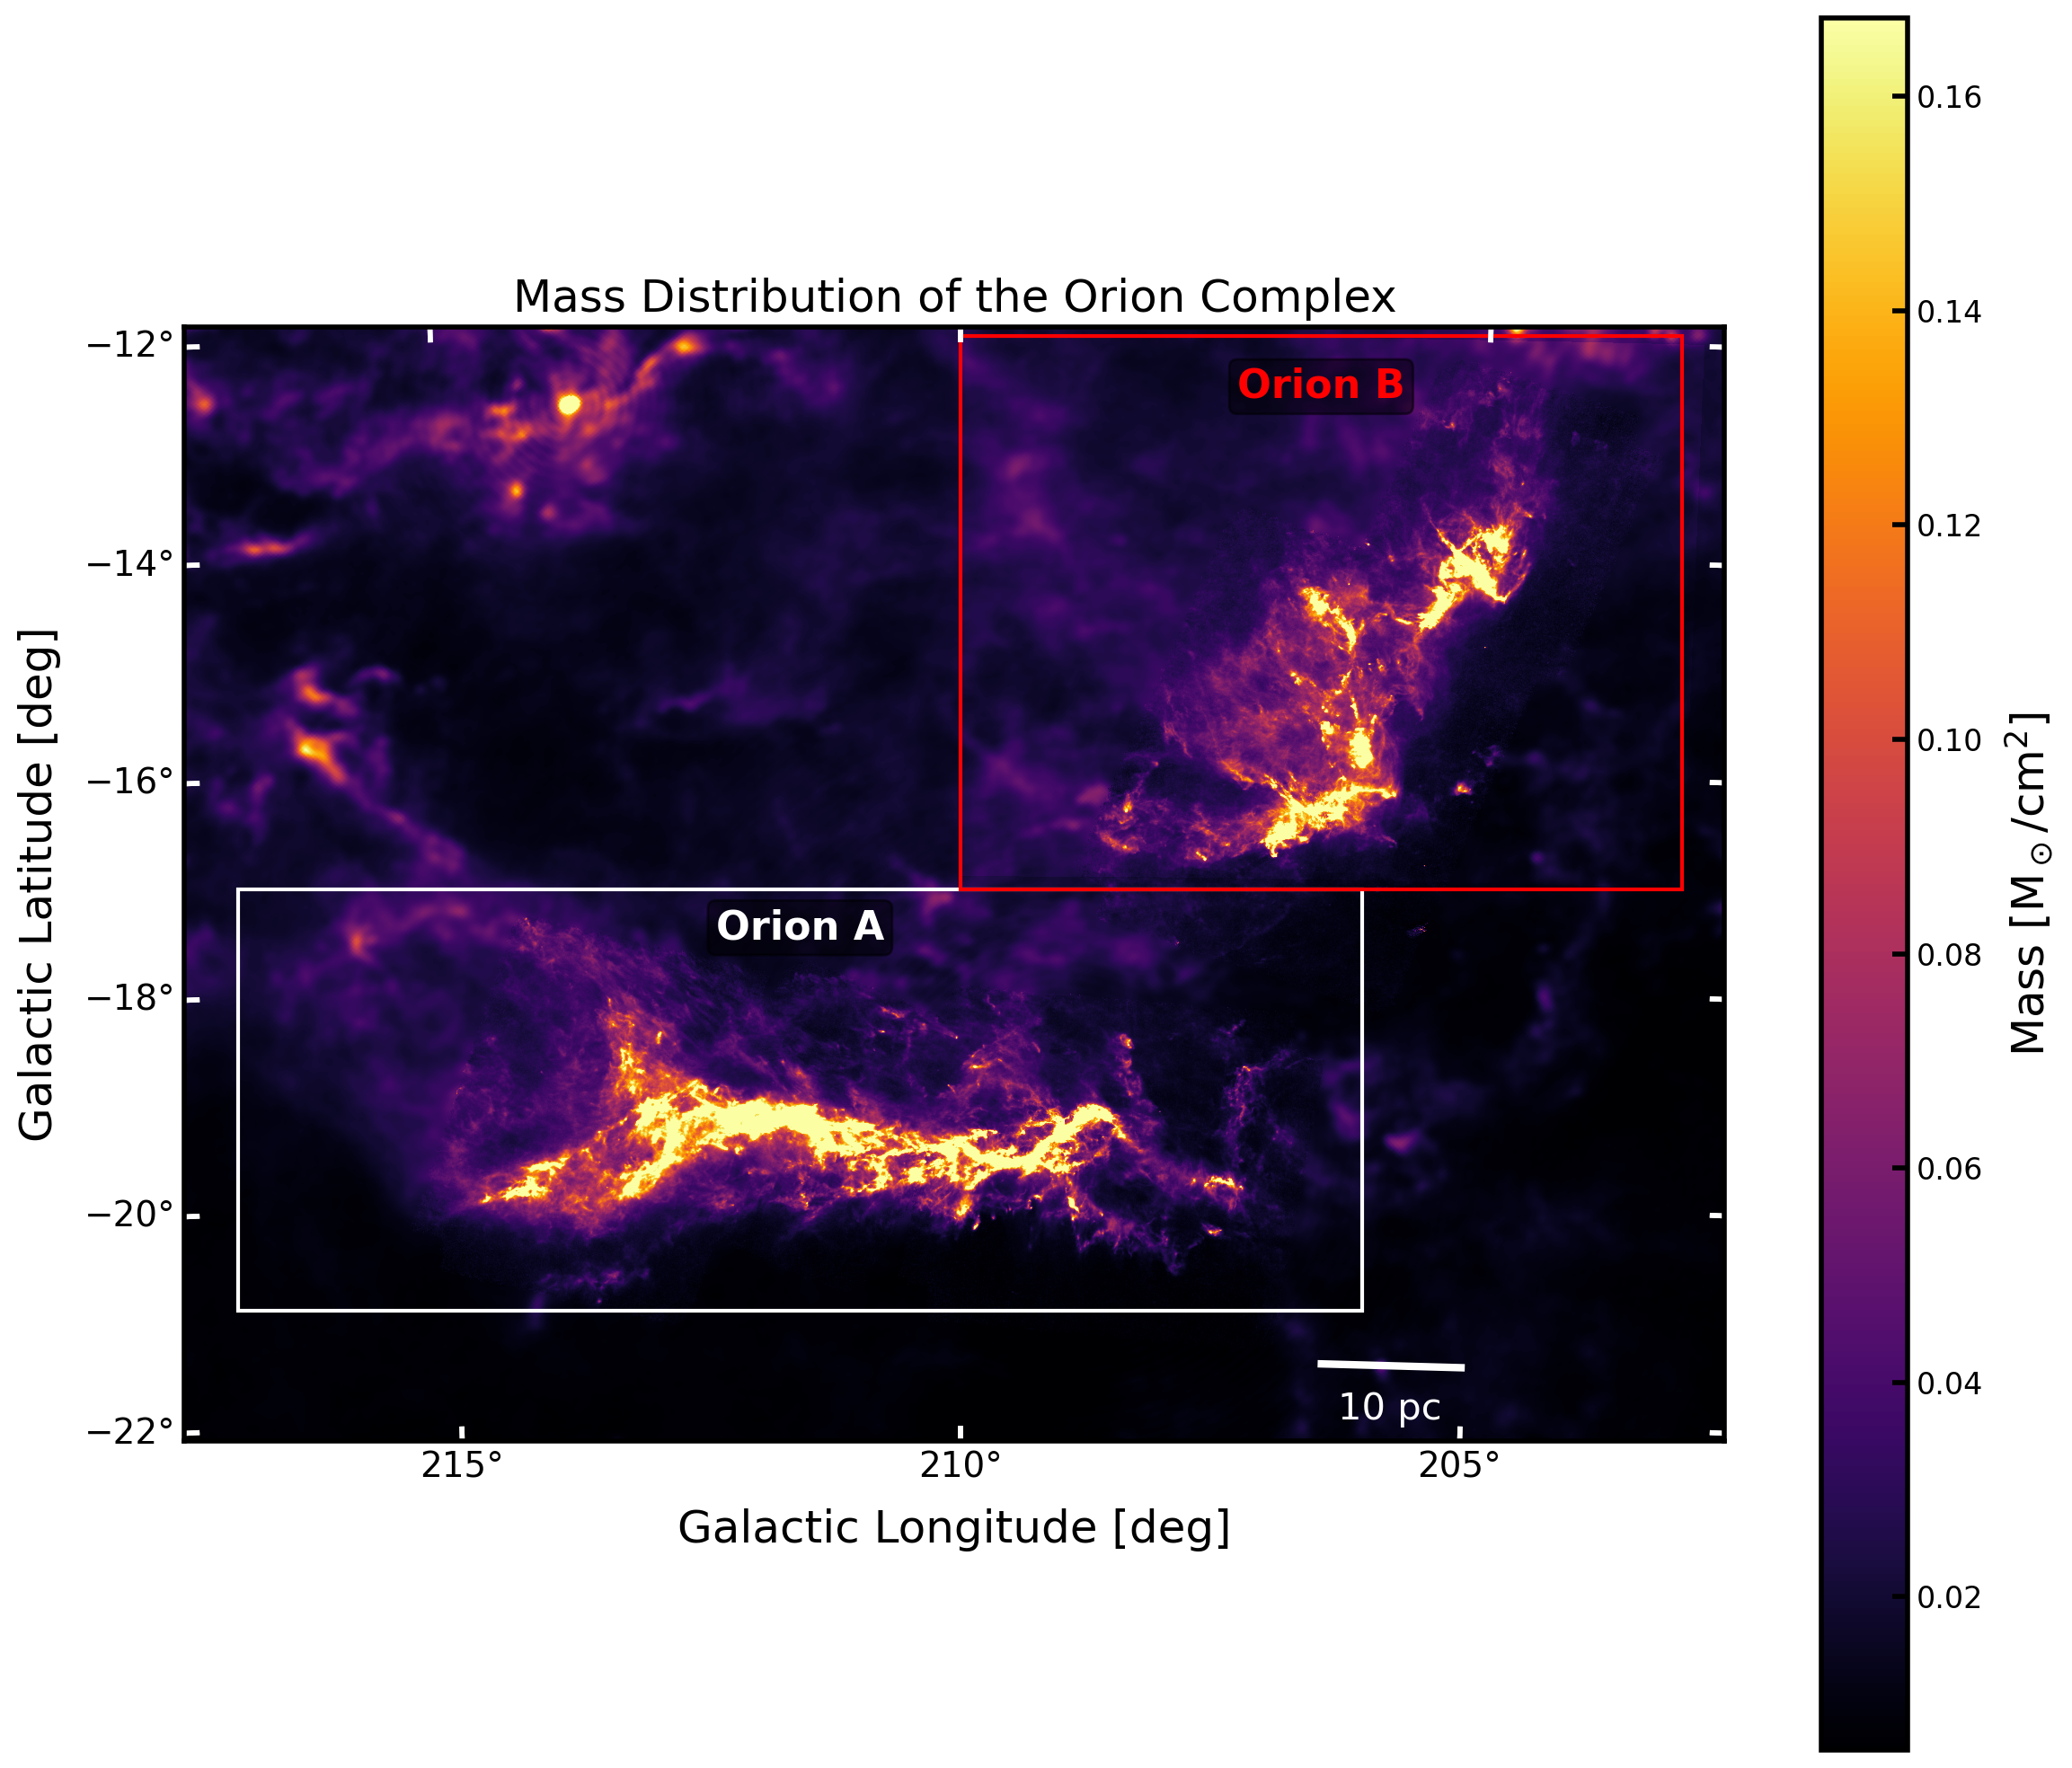
\includegraphics[width=0.75\textwidth]{figures/mass_distribution.png}
    \caption{Mass map of the Orion A and B molecular clouds derived from the H$_2$ column density maps. The map shows the total mass in solar masses contained in each pixel.}
    \label{fig:mass_map}
\end{figure}

The masses are computed by integrating the mass surface density over the spatial extent of each cloud, defined by fixed Galactic longitude ($\ell$) and latitude ($b$) boundaries:

\begin{itemize}
    \item Orion A: $206^\circ < \ell < 217^\circ$, $-21^\circ < b < -17^\circ$
    \item Orion B: $203^\circ < \ell < 210^\circ$, $-17^\circ < b < -12^\circ$
\end{itemize}

Using these definitions and the mass maps, we estimate the mass of Orion A to be approximately $8.62 \times 10^4 \, M_\odot$, the mass of Orion B to be approximately $7.02 \times 10^4 \, M_\odot$
The total mass of Orion A and B combined is therefore approximately $1.56 \times 10^5 \, M_\odot$.

\subsection{Data Pre-processing}

To ensure consistency and reliability in the derived column density and mass maps, several pre-processing steps were applied to both the original \textit{Herschel} data and the derived extinction products from \cite{lombardi2014herschel}. These steps aimed to isolate high-resolution structure, remove contaminating background emission, and maintain uniform calibration across the dataset.

The original \textit{Herschel} photometric maps used in the derivation of extinction and column density maps were processed using the Herschel Interactive Processing Environment (HIPE; \cite{mizumoto2010astronomical}), version 10.0.2843, along with the most up-to-date calibration files available at the time. Standard pipeline procedures were followed, including detector deglitching, baseline removal, and map-making.

Since the raw maps often contain large-scale background emission and lower-resolution contributions from the \textit{Planck} mission, a spatial filtering step was performed to isolate the high-resolution structure traced by \textit{Herschel}'s PACS and SPIRE instruments. Specifically, we masked the lower-resolution \textit{Planck}-dominated regions and retained only those spatial frequencies that correspond to \textit{Herschel}'s native angular resolution. This effectively removed diffuse Galactic foregrounds and background gradients, improving the contrast of compact and filamentary structures within the Orion A and B clouds.

The column density maps from \cite{lombardi2014herschel} were obtained by fitting a modified blackbody model to \textit{Herschel} data and calibrated using NIR extinction measurements via the NICEST/2MASS technique. These maps already incorporated several pre-processing steps, including spatial regridding, background subtraction, and convolution to a common beam size.

For our purposes, we applied additional masking to exclude low-signal or edge pixels where the uncertainty in the optical depth was high. These masks ensure that only high-confidence regions are used in the column density and mass derivations.

In summary, the pre-processing workflow ensures that:
\begin{itemize}
    \item Only high-resolution \textit{Herschel} data contribute to the final maps.
    \item Large-scale background emission is removed.
    \item Low signal-to-noise regions and unreliable pixels are masked out.
    \item Calibration and resolution across maps are homogenized.
\end{itemize}

These steps are essential for producing reliable maps of dust-derived column density and mass structure in the Orion molecular clouds.

% To-Do:
% some other properties of the YSO catalogue
% remake picture 
\section{Young Stellar Objects (YSOs)}

\subsection{Introduction}

Understanding the relationship between the internal structure of molecular clouds and their ability to form stars is a central goal of star formation studies. In this work, we investigate how the morphology and column density distribution of the Orion A and B clouds relate to their young stellar content. To this end, we utilize the Young Stellar Object (YSO) catalogue compiled by \cite{megeath2012catalogue}, which provides a detailed census of the star-forming population in Orion.

The catalogue is based on observations from the \textit{Spitzer Space Telescope}, specifically using data from the Infrared Array Camera (IRAC; \cite{fazio2004IRAC}) and the Multiband Imaging Photometer for Spitzer (MIPS; \cite{rieke2004MIPS}), covering approximately 9 deg$^2$ in five mid-infrared bands. These wavelengths are sensitive to warm dust and circumstellar material, allowing for the identification of young stars through their infrared excesses. The classification of YSOs is primarily based on the slope of their spectral energy distributions (SEDs) in the mid-infrared, following standard criteria.

Additionally, the catalogue incorporates near-infrared data from the 2MASS survey \cite{skrutskie2006two}, which helps to identify less embedded sources and complements the mid-infrared sensitivity.

\subsection{The catalogue}
The catalogue \footnote{\href{http://cdsarc.cds.unistra.fr}{YSO catalogue in the CDS Archive}} includes a total of 3479 dusty YSOs, classified primarily based on their spectral energy distributions (SEDs). These classifications distinguish between:
\begin{itemize}
    \item Protostars (P): deeply embedded sources with rising or flat SEDs, indicative of ongoing mass accretion (N=488).
    \item Disk sources (D): more evolved pre-main sequence stars that still retain circumstellar disks, but with declining mid-infrared emission (N=2991).
\end{itemize}

The YSO dataset provides key information for each object, including spatial coordinates, infrared luminosity, and evolutionary class. This makes it a powerful tracer of the recent and ongoing star formation within the Orion clouds.

A spatial overview of the YSO population is shown in Figure \ref{fig:YSO_map}, where the distribution of protostars and disk sources is overlaid on the column density map. This visualization allows for a direct comparison between the gas structure and the stellar content, enabling a statistical study of the relationship between dense gas and star-forming activity.

\begin{figure}[t]
    \centering
    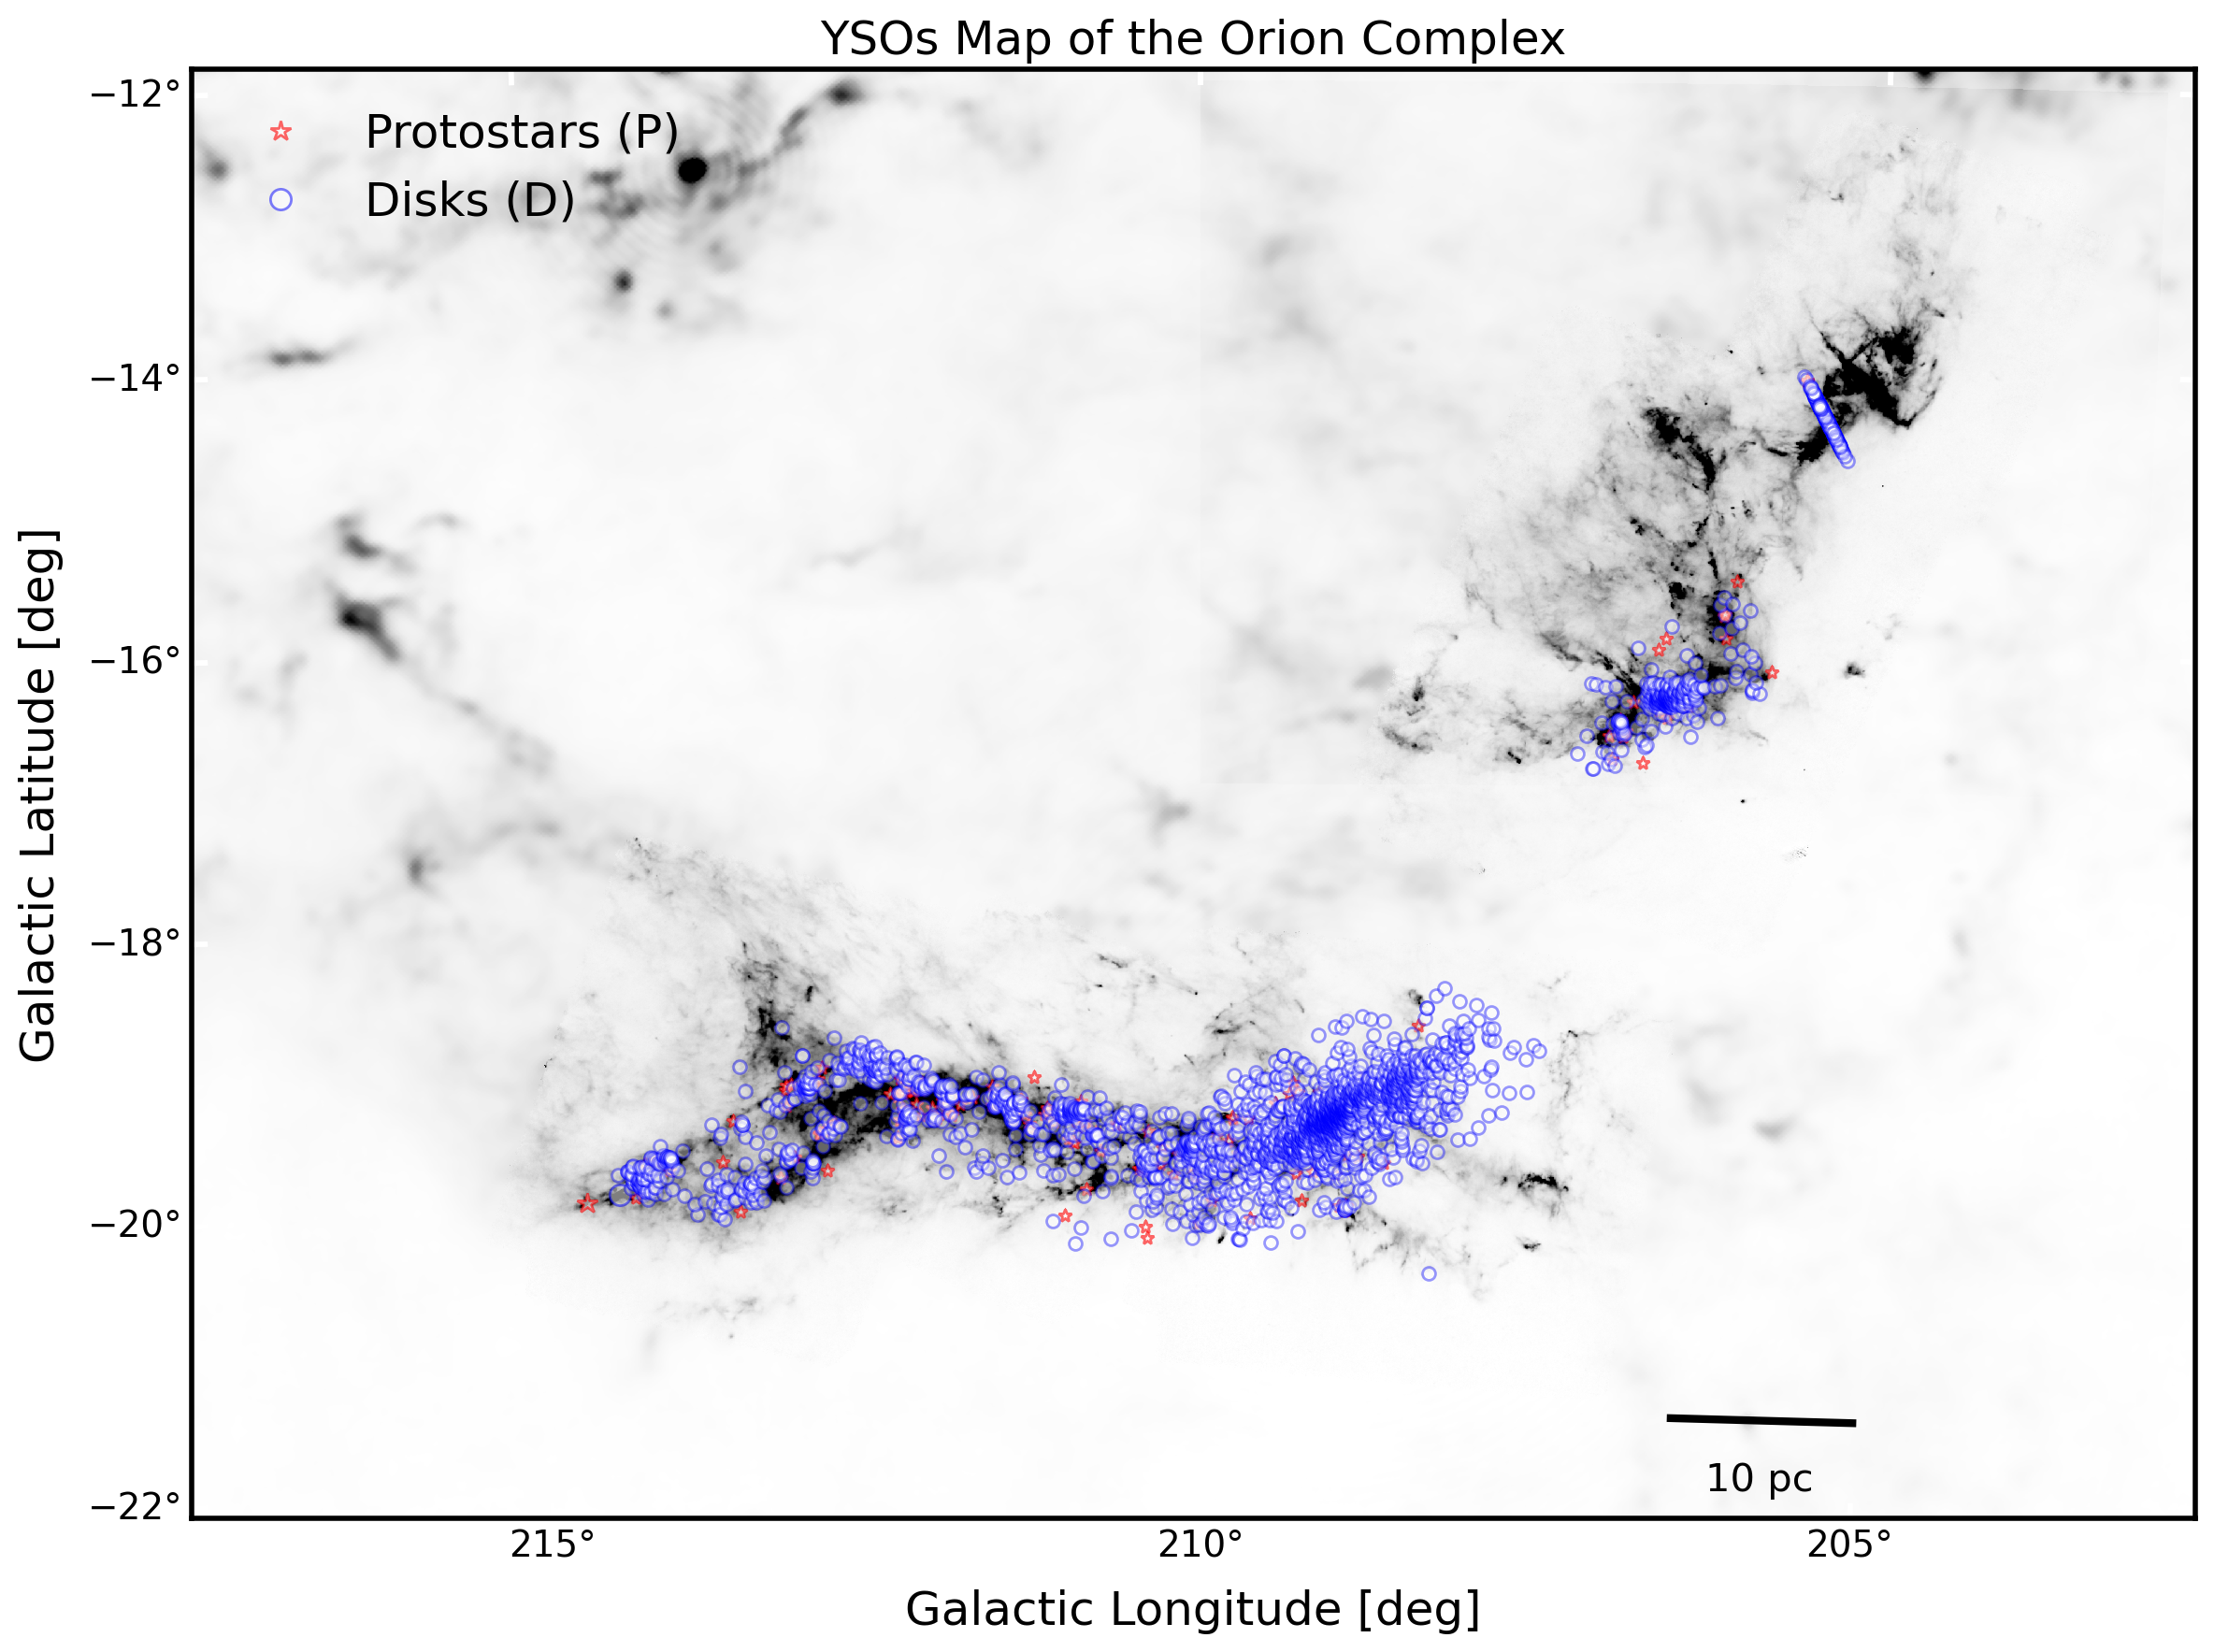
\includegraphics[width=0.85\textwidth]{figures/YSOs_orion.png}
    \caption{Map of YSOs in the Orion A and B clouds, overlaid on the column density map. YSOs are color-coded by evolutionary class, with protostars (P, red stars) and disk sources (D, blue circles) identified based on their mid-infrared spectral energy distributions.}
    \label{fig:YSO_map}
\end{figure}